\section{Исследовательская часть}

	Для взаимодействия с загружаемым модулем был разработана программа пользовательского режима. Её интерфейс представлен на рисунке \ref{demo:interface}.

	\begin{figure}[h!] 
		\begin{center}
			{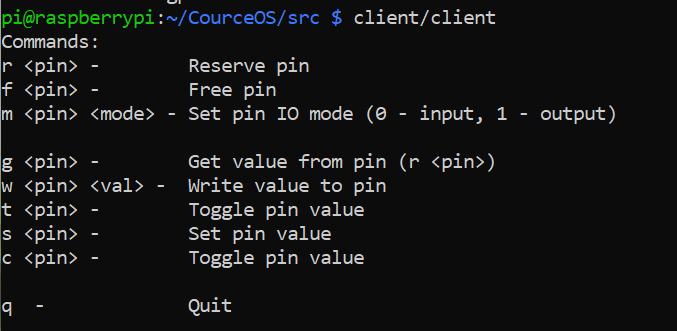
\includegraphics[scale=1.2, angle=0]{img/interface.png}}
			\caption{Интерфейс программы}
			\label{demo:interface}
		\end{center}
	\end{figure}

	Для тестирования работы программы к компьютеру были подключены реле и кнопка (номера контактов 17 и 22 соотвественно).
	
	Первым тестом является изменение состояния реле \ref{demo:test1}. В результате теста значение было успешно изменено - при установке логической единице на 17-м контакте реле было открыто.
	
	\begin{figure}[h!] 
		\begin{center}
			{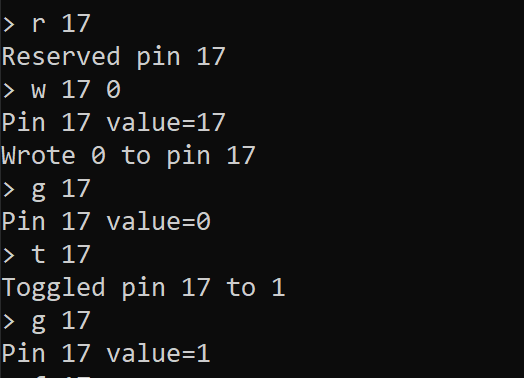
\includegraphics[scale=1.0, angle=0]{img/test1.png}}
			\caption{Тест вывода}
			\label{demo:test1}
		\end{center}
	\end{figure}

	Вторым тестом является проверка изменения значения при нажатии кнопки \ref{demo:test2}. В результате теста считываемое значение было изменено во время зажатия кнопки.
	
	\begin{figure}[h!] 
		\begin{center}
			{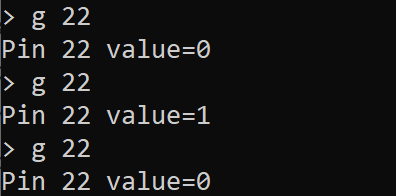
\includegraphics[scale=1.0, angle=0]{img/test2.png}}
			\caption{Тест ввода}
			\label{demo:test2}
		\end{center}
	\end{figure}

	Третьим тестом является проверка контроля захвата управления контактами \ref{demo:test3}. Действия выполняются сначала в правом терминале, потом в левом. Как можно видеть, операция чтения позволена без захвата контроля. При попытке второго процесса захватить управление или совершить операцию вывода на уже используемый пин, ему возвращается ошибка.
	
	\begin{figure}[h!] 
		\begin{center}
			{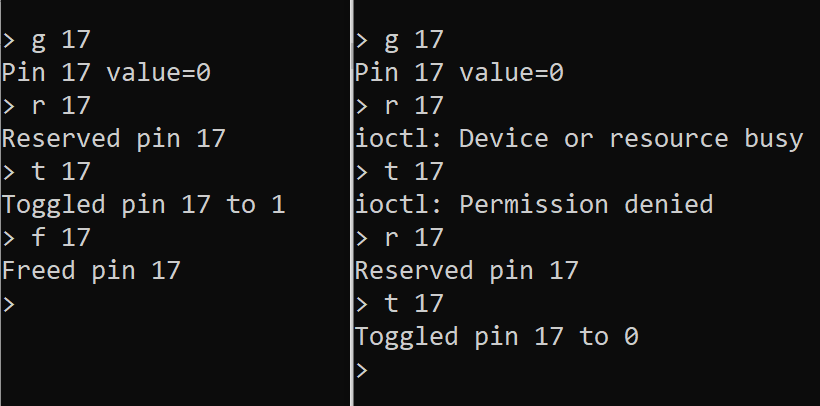
\includegraphics[scale=1.0, angle=0]{img/test3.png}}
			\caption{Тест контроля захвата и возвращения управления}
			\label{demo:test3}
		\end{center}
	\end{figure}

\pagebreak